\documentclass{article}

\title{Notes: Stretch Mapping}
\author{D. Fang}
\date{\today}

\usepackage{amsmath}
\usepackage{derivative}
\usepackage{tikz}
\usepackage{tcolorbox}

\newcommand{\me}{m_\mathrm{e}}
\newcommand{\mpr}{m_\mathrm{p}}
\newcommand{\mue}{\mu_\mathrm{e}}
\newcommand{\tpf}{\tilde{p}_F}
\newcommand{\Mtot}{M_{\text{tot}}}
\newcommand{\xmax}{x_{\max}}
\newcommand{\dr}{\odif{r}}
\newcommand{\Rsun}{R_{\odot}}
\newcommand{\Msun}{M_{\odot}}

\DeclareMathOperator{\arcsinh}{arcsinh}
\DeclareMathOperator{\sinc}{sinc}

\begin{document}

\maketitle
\tableofcontents

\section{Coordonnées}

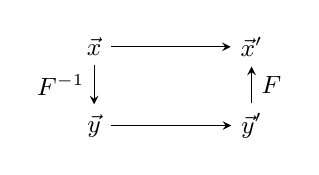
\begin{tikzpicture}[node distance=2cm, >=stealth, every node/.style={font=\small}]

  % positions
  \node (a) at (0,1) {$\vec x$};
  \node (b) at (0,0) {$\vec y$};
  \node (c) at (2,0) {$\vec y'$};
  \node (d) at (2,1) {$\vec x'$};

  % arrows
  \draw[->] (a) -- (b) node[midway, left] {$F^{-1}$};                     % a -> b (down)
  \draw[->] (b) -- (c);                     % b -> c (right)
  \draw[->] (c) -- (d) node[midway, right] {$F$};   % c -> d (up) with label
  \draw[->] (a) -- (d);                     % a -> d

\end{tikzpicture}

La procédure de stretch mapping permet d'obtenir les 3 composantes $\vec y'$ à partir de celles de $\vec y$ de manière indépendante.
\[ y_i' = \xi_i(y_i) \]
On veut ensuite retrouver les composantes dans la base de $\vec x$.
Souvent les changements de bases se factorisent, dans le sens où
\begin{equation}
  x_i = \prod_j F^j_i(y_j)
  \label{eq:initial}
\end{equation}
Par exemple,
\begin{align*}
  x &= r \cos\theta\sin\phi
  \\
  y &= r \sin\theta\sin\phi
  \\
  z &= r\cos\phi
\end{align*}

Donc
\begin{align*}
  x_i' &= \prod_j F^j_i(y_j') \\
  &= \prod_j F^j_i(\xi_j(y_j))
\end{align*}
Le problème ainsi c'est que l'on réalise souvent des étapes en trop. Par exemple si on stretch seulement selon $r$, alors il faut partir de $(x,y,z)$, obtenir  $(r,\theta,\phi)$ puis $(r',\theta,\phi)$ puis revenir à $(x',y',z')$. Le calcul de $\theta$ et $\phi$ est alors inutile puisqu'ils restent inchangés.

Dans ce cas, il suffit de suivre la procédure suivante. On part en fait de \eqref{eq:initial} et on l'injecte dans

\section{Introduction}
On cherche un potentiel pour contrer la pression.

\[ -\nabla P + \nabla \phi_{\text{fictif}} =0 \]
On parle d'équation localement isotherme lorsque la température dépend uniquement de la position. Elle est prescrite. Dans les disques protoplanétaires, on dit en effet qu'elle dépend de la distance à l'étoile.

Eos adiabatique :
\[ \rho = P^\gamma \]

\section{Smoothing length}
On veut imposer
\[ h_a = h_{\text{fact}}\left(\frac{m_a}{\rho_a}\right)^(1/3) \]
Or on donne $ \rho_{\text{profile}}$ tel que
\[ \rho(r) = m_{\text{tot}}   \frac{\rho_{\text{profile}}(r)}{\int_{r_{\min}}^{r_{\max}} \rho_{\text{profile}}(r) \odif{S} \odif{r}}\]

\section{HCP Lattice}
On a un cube dans lequel on place des cellules unités hcp. Chaque cellule est de volume $24\sqrt{2}r$ donc au total on a $\frac{(2\xmax)^3}{24\sqrt{2}r}$ cellules. Chaque cellule a 6 atomes donc il reste
\[
  \frac{(2\xmax)^3}{4\sqrt{2}\dr^3} \text{ atomes}
\]
Enfin on crop une sphère donc il reste
\[
  N = \frac{(2\xmax)^3}{4\sqrt{2}\dr^3} \times \frac{\frac43 \pi \xmax^3}{(2\xmax)^3} \text{ atomes}
\]
Dans Shamrock on entre la masse d'une particule:
\[ m_{\text{part}} = \frac{M_{\text{tot}}}{N} \]
où $M_{\text{tot}}$ est la masse de l'étoile que l'on souhaite.
Mais ce serait plus pratique d'entrer $(\Mtot, N, \xmax)$ et d'en déduire $\dr$. On inverse donc
\[ \dr = 2\xmax\left[\frac{1}{4\sqrt2 N}\times\frac{\frac43 \pi}{2^2} \right]^{\frac13}\]

\subsection{Relation masse rayon}
On veut connaître maintenant le lien entre xmax et la masse totale de l'étoile puisqu'a la fin on ne précise que xmax et dr.
Le rayon d'une naine blanche est celle qui maximise ? l'energie libre ?
\[
R_* = \frac{(9\pi)^{2/3}}{8} \frac{\hbar^2}{\me} \frac{1}{G m_p^{5/3} M_{\text{tot}}^{1/3}}\]

\[
  \frac{R_*}{\Rsun} = 0.010\left( \frac{\Msun}{\Mtot}\right)^{\frac13}
\]
Plus l'étoile est massive, plutôt elle doit être petite.

\subsection{Polytrope}
Pour une étoile polytropique. On suit la même procédure. On impose la masse, le rayon est alors contraint.

On donne $\Mtot, \tilde\rho$.
Alors avant de démarrer la procédure de stretch mapping il faut connaître le rayon.
\[
  \Mtot = \int_{0}^{R} \rho_c \tilde\rho(r)4\pi\odif{r}^2
\]
mais donc il faut connaître $\rho_c$. Il nous faut une 2ème équation. Le profil de densité, peu importe son facteur de normalisation doit s'annuler en $R$.
\[
  \tilde \rho(R) = 0
\]
ce qui impose $R$. On pourrait croire que cette équation suffit pour avoir $R$. Mais en fait $\rho_c$ apparaît dedans en raison de l'adimensionnement des équations de Lane-Emden
\[  \tilde \rho(r) = \sinc(\xi(r,\rho_c))\]
avec
\[ \xi(r,\rho_c) =  r\sqrt{\frac{4\pi G\rho_c^2}{(n+1)P_c}} =  r\sqrt{\frac{4\pi G\rho_c^{1-\frac1n}}{(n+1)K}}\]
Finalement, le couple d'équations est
\begin{align}
  0 &=  \tilde \rho(R, \rho_c) \\
  \Mtot &= \int_{0}^{R} \rho_c \tilde\rho(r)4\pi\odif{r}^2
\end{align}
En particulier pour $n=2$,
\[
0 = \sinc\left(R\sqrt{\frac{2\pi G}{K}}\right) \quad \textit{(on a de la chance que $\rho_c$ disparaisse...)} \]
\begin{align*}
  R &= \sqrt{\frac{\pi K}{2 G}} \\
  \Mtot &= \rho_c \int_{0}^{\sqrt{\frac{\pi K}{2 G}}}  \tilde\rho(r)4\pi\odif{r}^2
\end{align*}
tl:dr. Pour $n=1$, c'est la valeur de $K$ uniquement qui impose le rayon. La seule chose qu'on impose c'est $\Mtot$ (donc $N_{\text{part}}, m_{\text{part}}$). $\rho_c$ n'a aucune importance ici.

Résumé :
\begin{itemize}
  \item Fermi : On impose $\Mtot$ ce qui contraint $R$ directement.
  \item Polytrope : On impose $K,n=1$ ce qui contraint $R$. Puis $\Mtot$ arrive en dernier. Sinon on peut faire l'inverse : imposer $R$ ce qui contraint $K$.
\end{itemize}
% \[ R_*^{\text{polytrop}} = \sqrt{\frac{\pi K}{2G}} \]
% En fait en général
% \[ R_*^{\text{polytrop}} = \sqrt{\frac{(n+1)P_c}{4\pi G \rho_c^2}}\xi_1 \]
% $\xi_1$ étant le point où la densité s'annule.
% avec
% \[ \xi = r\sqrt{\frac{4\pi G\rho_c^2}{(n+1)P_c}} \]

\section{Équations d'état}
\subsection{Fermi}

Par définition de la vitesse du son
\[ c_s^2 \equiv \pdv{P}{\rho} \]
Dans le cas de Fermi,
\[ c_s^2 = \pdv{P}{\tpf}\pdv{\tpf}{\rho}\]
avec
\begin{align*}
  \tpf &= \frac{1}{\mue^{\frac13}}\alpha \rho^{1/3} \\
  P &= \beta \left(\left[\tpf\sqrt{\tpf^2+1}(2\tpf^2-3)+3\arcsinh(\tpf)\right]\right)
\end{align*}
et
\begin{align*}
  \alpha &= \frac{1}{\me c}h\left(\frac{3}{8\pi m_{\mathrm{p}}}\right)^{\frac13} \\
  \beta &= \frac{\pi m_\mathrm{e}^4c^5}{3h^3}
\end{align*}
Donc chaque dérivée donne
\begin{align*}
  \pdv{\tpf}{\rho} &= \frac{1}{3\mue^{\frac13} }\alpha\rho^{\frac13-1} \\
  \pdv{P}{\tpf} &= \beta\Bigg\{\sqrt{\tpf^2+1}(2\tpf^2-3) + \tpf\left[\frac{\tpf}{\sqrt{\tpf^2+1}}(2\tpf^2-3) + 4\tpf\sqrt{\tpf^2+1}\right]  \\
  & \quad + \frac{3}{\sqrt{1+\tpf^2}} \Bigg\} \\
  &= \beta\Bigg\{\frac{1}{\sqrt{1+\tpf^2}}\Bigg[\underbrace{(2\tpf^2-3)(1+\tpf^2)}_{-\tpf^2 + 2\tpf^4 - 3}+ \tpf^2\underbrace{\left[2\tpf^2-3 + 4(\tpf^2+1)\right]}_{6\tpf^2+1}\Bigg]
  + \frac{3}{\sqrt{1+\tpf^2}} \Bigg\} \\
  &= \beta\Bigg\{\frac{8\tpf^4 -3}{\sqrt{1+\tpf^2}}
  + \frac{3}{\sqrt{1+\tpf^2}} \Bigg\} \\
  &= \beta\frac{8\tpf^4}{\sqrt{1+\tpf^2}}
\end{align*}
Finalement
\[ c_s^2 = \frac{8\alpha\beta}{3\mue^{\frac13}\rho^{\frac23}}\frac{\tpf^4}{\sqrt{1+\tpf^2}}\]

\begin{tcolorbox}
  \begin{align*}
    P &= \beta \left(\left[\tpf\sqrt{\tpf^2+1}(2\tpf^2-3)+3\arcsinh(\tpf)\right]\right)\\
    c_s^2 &= \frac{8\alpha\beta}{3\mue^{\frac13}\rho^{\frac23}}\frac{\tpf^4}{\sqrt{1+\tpf^2}}
  \end{align*}
  with
  \begin{align*}
    \tpf &= \frac{1}{\mue^{\frac13}}\alpha \rho^{1/3} \\
    \alpha &= \frac{1}{\me c}h\left(\frac{3}{8\pi m_{\mathrm{p}}}\right)^{\frac13} \\
    \beta &= \frac{\pi m_\mathrm{e}^4c^5}{3h^3}
  \end{align*}
\end{tcolorbox}

\section{Equation de Chandrasekhar}

\[
  \frac{1}{\eta^2} \odv{}{\eta} \left( \eta^2 \odv{\Phi}{\eta} \right) = - \left( \Phi^2 - \frac{1}{y_0^2} \right)^{3/2}
\]

Conditions aux limites :
\begin{align*}
  \Phi(0) &= 1 \\
  \Phi'(0) &= 0 \\
\end{align*}

On résout numériquement cette équation puis on repasse dans les bonnes dimensions.

\begin{align*}
  \eta &= \frac{r}{a} \\
  \Phi &= \frac{1}{y_0}\sqrt{1+\frac{\rho}{C}^{\frac23}}
\end{align*}
On inverse
\begin{align*}
  r &= a\eta \\
  \rho &= C\left[(y_0\Phi)^2- 1\right]^{\frac32}
\end{align*}
Les constantes valent
\begin{align*}
  C &= \frac{8\pi\me^3c^3\mpr}{3h^3} \mue = C_1\mue \\
  a &= \frac{1}{C y_0}\sqrt{\frac{2\beta}{\pi G}} = r_a\frac{1}{\mue y_0}
\end{align*}
avec
\[
  r_a = \frac{1}{C_1}\sqrt{\frac{2\beta}{\pi G}}
\]

\end{document}
